% Generated by ArticleSignalDiagrams. Opaque vector fills only.
\documentclass[10pt,tikz,border=5pt]{standalone}
\usepackage{lmodern}
\usetikzlibrary{fit}
\begin{document}
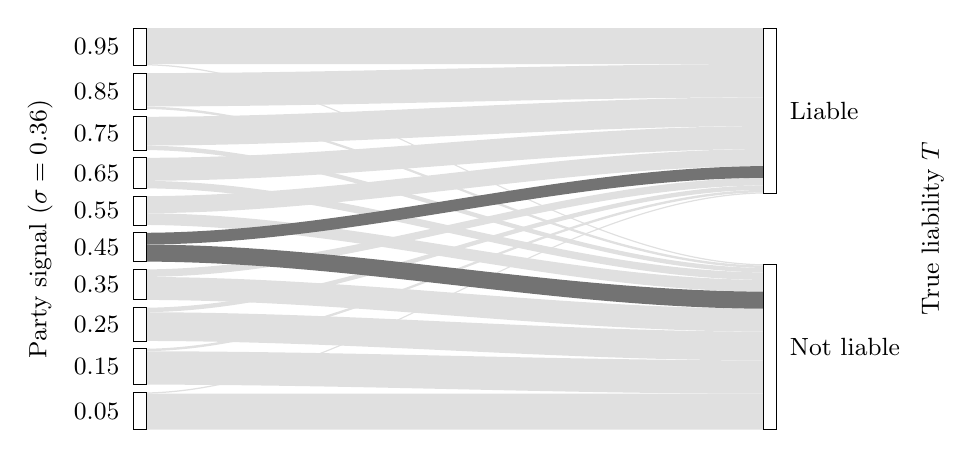
\begin{tikzpicture}[x=1cm,y=1cm,font=\small]\path[fill=black!12,draw=none] (3.3,-5.1) .. controls (6,-5.1) and (8.6,-5.1) .. (11.3,-5.1) -- (11.3,-4.643759) .. controls (8.6,-4.643759) and (6,-4.643759) .. (3.3,-4.643759) -- cycle;
\path[fill=black!12,draw=none] (3.3,-4.643759) .. controls (6,-4.643759) and (8.6,-2.1) .. (11.3,-2.1) -- (11.3,-2.084116) .. controls (8.6,-2.084116) and (6,-4.627875) .. (3.3,-4.627875) -- cycle;
\path[fill=black!12,draw=none] (3.3,-4.527875) .. controls (6,-4.527875) and (8.6,-4.643759) .. (11.3,-4.643759) -- (11.3,-4.22032) .. controls (8.6,-4.22032) and (6,-4.104436) .. (3.3,-4.104436) -- cycle;
\path[fill=black!12,draw=none] (3.3,-4.104436) .. controls (6,-4.104436) and (8.6,-2.084116) .. (11.3,-2.084116) -- (11.3,-2.053026) .. controls (8.6,-2.053026) and (6,-4.073346) .. (3.3,-4.073346) -- cycle;
\path[fill=black!12,draw=none] (3.3,-3.973346) .. controls (6,-3.973346) and (8.6,-4.22032) .. (11.3,-4.22032) -- (11.3,-3.855581) .. controls (8.6,-3.855581) and (6,-3.608607) .. (3.3,-3.608607) -- cycle;
\path[fill=black!12,draw=none] (3.3,-3.608607) .. controls (6,-3.608607) and (8.6,-2.053026) .. (11.3,-2.053026) -- (11.3,-1.996549) .. controls (8.6,-1.996549) and (6,-3.55213) .. (3.3,-3.55213) -- cycle;
\path[fill=black!12,draw=none] (3.3,-3.45213) .. controls (6,-3.45213) and (8.6,-3.855581) .. (11.3,-3.855581) -- (11.3,-3.563994) .. controls (8.6,-3.563994) and (6,-3.160543) .. (3.3,-3.160543) -- cycle;
\path[fill=black!12,draw=none] (3.3,-3.160543) .. controls (6,-3.160543) and (8.6,-1.996549) .. (11.3,-1.996549) -- (11.3,-1.901335) .. controls (8.6,-1.901335) and (6,-3.065329) .. (3.3,-3.065329) -- cycle;
\path[fill=black!12,draw=none] (3.3,-2.5) .. controls (6,-2.5) and (8.6,-3.347646) .. (11.3,-3.347646) -- (11.3,-3.198665) .. controls (8.6,-3.198665) and (6,-2.351019) .. (3.3,-2.351019) -- cycle;
\path[fill=black!12,draw=none] (3.3,-2.351019) .. controls (6,-2.351019) and (8.6,-1.752354) .. (11.3,-1.752354) -- (11.3,-1.536006) .. controls (8.6,-1.536006) and (6,-2.134671) .. (3.3,-2.134671) -- cycle;
\path[fill=black!12,draw=none] (3.3,-2.034671) .. controls (6,-2.034671) and (8.6,-3.198665) .. (11.3,-3.198665) -- (11.3,-3.103451) .. controls (8.6,-3.103451) and (6,-1.939457) .. (3.3,-1.939457) -- cycle;
\path[fill=black!12,draw=none] (3.3,-1.939457) .. controls (6,-1.939457) and (8.6,-1.536006) .. (11.3,-1.536006) -- (11.3,-1.244419) .. controls (8.6,-1.244419) and (6,-1.64787) .. (3.3,-1.64787) -- cycle;
\path[fill=black!12,draw=none] (3.3,-1.54787) .. controls (6,-1.54787) and (8.6,-3.103451) .. (11.3,-3.103451) -- (11.3,-3.046974) .. controls (8.6,-3.046974) and (6,-1.491393) .. (3.3,-1.491393) -- cycle;
\path[fill=black!12,draw=none] (3.3,-1.491393) .. controls (6,-1.491393) and (8.6,-1.244419) .. (11.3,-1.244419) -- (11.3,-0.87968) .. controls (8.6,-0.87968) and (6,-1.126654) .. (3.3,-1.126654) -- cycle;
\path[fill=black!12,draw=none] (3.3,-1.026654) .. controls (6,-1.026654) and (8.6,-3.046974) .. (11.3,-3.046974) -- (11.3,-3.015884) .. controls (8.6,-3.015884) and (6,-0.995564) .. (3.3,-0.995564) -- cycle;
\path[fill=black!12,draw=none] (3.3,-0.995564) .. controls (6,-0.995564) and (8.6,-0.87968) .. (11.3,-0.87968) -- (11.3,-0.456241) .. controls (8.6,-0.456241) and (6,-0.572125) .. (3.3,-0.572125) -- cycle;
\path[fill=black!12,draw=none] (3.3,-0.472125) .. controls (6,-0.472125) and (8.6,-3.015884) .. (11.3,-3.015884) -- (11.3,-3) .. controls (8.6,-3) and (6,-0.456241) .. (3.3,-0.456241) -- cycle;
\path[fill=black!12,draw=none] (3.3,-0.456241) .. controls (6,-0.456241) and (8.6,-0.456241) .. (11.3,-0.456241) -- (11.3,-0) .. controls (8.6,-0) and (6,-0) .. (3.3,-0) -- cycle;
\path[fill=black!55,draw=none] (3.3,-2.965329) .. controls (6,-2.965329) and (8.6,-3.563994) .. (11.3,-3.563994) -- (11.3,-3.347646) .. controls (8.6,-3.347646) and (6,-2.748981) .. (3.3,-2.748981) -- cycle;
\path[fill=black!55,draw=none] (3.3,-2.748981) .. controls (6,-2.748981) and (8.6,-1.901335) .. (11.3,-1.901335) -- (11.3,-1.752354) .. controls (8.6,-1.752354) and (6,-2.6) .. (3.3,-2.6) -- cycle;
\coordinate (axis-midline-0) at (0,-2.55);
\path[fill=white,draw=black,line width=0.3pt] (3.22,-5.1) rectangle (3.38,-4.627875);
\node[anchor=east,fill=white,inner sep=2pt] (bucket-0-0-0) at (3.12,-4.863937) {0.05};
\path[fill=white,draw=black,line width=0.3pt] (3.22,-4.527875) rectangle (3.38,-4.073346);
\node[anchor=east,fill=white,inner sep=2pt] (bucket-0-0-1) at (3.12,-4.30061) {0.15};
\path[fill=white,draw=black,line width=0.3pt] (3.22,-3.973346) rectangle (3.38,-3.55213);
\node[anchor=east,fill=white,inner sep=2pt] (bucket-0-0-2) at (3.12,-3.762738) {0.25};
\path[fill=white,draw=black,line width=0.3pt] (3.22,-3.45213) rectangle (3.38,-3.065329);
\node[anchor=east,fill=white,inner sep=2pt] (bucket-0-0-3) at (3.12,-3.258729) {0.35};
\path[fill=white,draw=black,line width=0.3pt] (3.22,-2.965329) rectangle (3.38,-2.6);
\node[anchor=east,fill=white,inner sep=2pt] (bucket-0-0-4) at (3.12,-2.782664) {0.45};
\path[fill=white,draw=black,line width=0.3pt] (3.22,-2.5) rectangle (3.38,-2.134671);
\node[anchor=east,fill=white,inner sep=2pt] (bucket-0-0-5) at (3.12,-2.317336) {0.55};
\path[fill=white,draw=black,line width=0.3pt] (3.22,-2.034671) rectangle (3.38,-1.64787);
\node[anchor=east,fill=white,inner sep=2pt] (bucket-0-0-6) at (3.12,-1.841271) {0.65};
\path[fill=white,draw=black,line width=0.3pt] (3.22,-1.54787) rectangle (3.38,-1.126654);
\node[anchor=east,fill=white,inner sep=2pt] (bucket-0-0-7) at (3.12,-1.337262) {0.75};
\path[fill=white,draw=black,line width=0.3pt] (3.22,-1.026654) rectangle (3.38,-0.572125);
\node[anchor=east,fill=white,inner sep=2pt] (bucket-0-0-8) at (3.12,-0.79939) {0.85};
\path[fill=white,draw=black,line width=0.3pt] (3.22,-0.472125) rectangle (3.38,-0);
\node[anchor=east,fill=white,inner sep=2pt] (bucket-0-0-9) at (3.12,-0.236063) {0.95};
\node[fit=(bucket-0-0-0) (bucket-0-0-1) (bucket-0-0-2) (bucket-0-0-3) (bucket-0-0-4) (bucket-0-0-5) (bucket-0-0-6) (bucket-0-0-7) (bucket-0-0-8) (bucket-0-0-9),inner sep=0pt] (source-labels-0) {};
\coordinate (axis-title-0-0) at (source-labels-0.west |- axis-midline-0);
\node[rotate=90,anchor=south,inner sep=0pt] at ([xshift=-0.18cm]axis-title-0-0) {Party signal ($\sigma=0.36$)};
\path[fill=white,draw=black,line width=0.3pt] (11.22,-5.1) rectangle (11.38,-3);
\node[anchor=west,fill=white,inner sep=2pt] (bucket-0-1-0) at (11.48,-4.05) {Not liable};
\path[fill=white,draw=black,line width=0.3pt] (11.22,-2.1) rectangle (11.38,-0);
\node[anchor=west,fill=white,inner sep=2pt] (bucket-0-1-1) at (11.48,-1.05) {Liable};
\node[fit=(bucket-0-1-0) (bucket-0-1-1),inner sep=0pt] (destination-labels-0) {};
\coordinate (axis-title-0-1) at (destination-labels-0.east |- axis-midline-0);
\node[rotate=90,anchor=north,inner sep=0pt] at ([xshift=0.18cm]axis-title-0-1) {True liability $T$};
\end{tikzpicture}
\end{document}

